Es ist wichtig bei allen folgenden Sequenzdiagrammen zu beachten, dass die sonst als lifelines bekannten Objekte hier als "usageline" interpretiert werden sollten.

\section{SuS-Login}
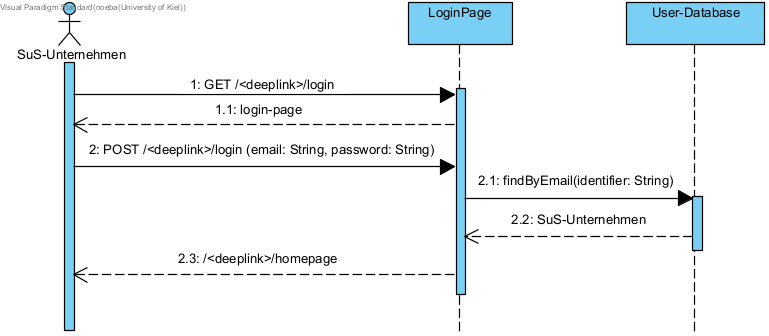
\includegraphics[width=\textwidth]{img/sequence-sus-login}
\label{fig: SuS-Login Sequenzdiagramm}
Um sich als SuS-Unternehmen einzuloggen wird vom oder von der Nutzer*in erst die LoginPage via Deeplink abgefragt. An diese werden danach die Logindaten gesendet, welche diese weiter an die Datenbank leitet um den oder die Nutzer*in zu authentifizieren. Ist die Authentifikation erfolgreich, so gibt die Datenbank den SuS-Unternehmen-Account zurück an die LoginPage und diese leitet den oder die Nutzer*in weiter zu der Shop-Homepage.

\section{SuS Produkt kaufen}
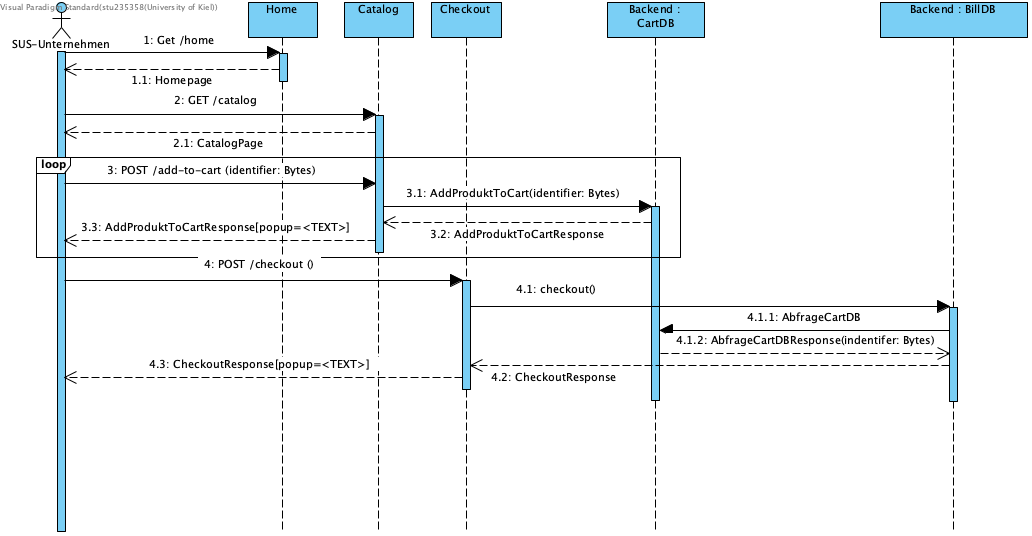
\includegraphics[width=\textwidth]{img/sequence-sus-buy-product}
\label{fig: SuS Produkt kaufen Sequenzdiagramm}
Dieses Sequenzdiagramm beschreibt den Prozess vom Produkt anschauen bis hin zum Kauf. Nachdem der oder die Nutzer*in die Homepage abgefragt und erhalten hat, fragt diese*r die Katalogsseite ab. Hier kann nun ein Produkt in Warenkorb hinzugefügt werden. Produkt \& session werden an eine Backend-Komponente weitergeleitet, welche den aktuellen Warenkorb für jeden Nutzer speichert. Werden mehr als nur eine Instanz des Produkts gleichzeitig dem Warenkorb hinzugefügt, so wird dieser loop entsprechend oft durchgeführt. Entscheidet sich der oder die Nutzer*in den Warenkorb zu bestellen, so schickt er/sie über die Weboberfläche einen Anfrage an einen Checkout-Endpoint, welcher diese and die Bill-Datenbank im Backend sendet. Die Bill-Datenbank fragt dann bei der Cart-Datenbank an, welche Objekte sich im Warenkorb befinden und generiert eine Rechnung, welche gespeichert und an den Nutzer zurückgeschickt wird.

\section{Lehrkraft Produkt hinzufügen}
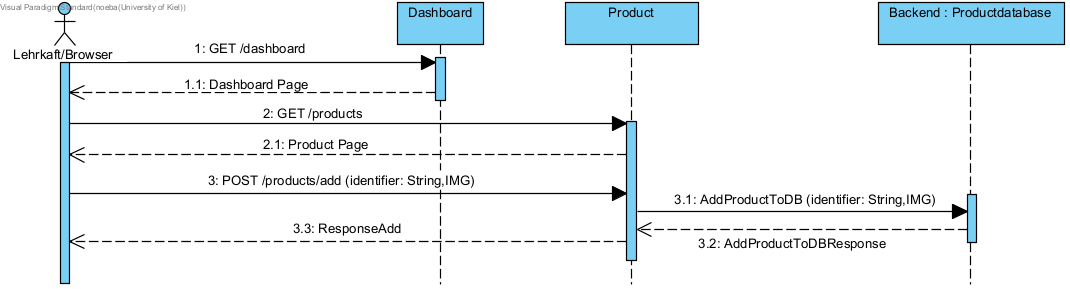
\includegraphics[width=\textwidth]{img/sequence-lehrkraft-add-product}
\label{fig: Lehrkraft Produkt hinzufügen Sequenzdiagramm}
Wir zeigen hier den Sequenzablauf für eine Lehrkraft, die ein Produkt ins System einführen möchte.\\
Nach dem Login und dem navigieren zur Produkt-Hinzufügungs-Oberfläche folgen über POST die Daten über das Produkt. Die Lehrkraft wird dann wieder auf die Ursprungsseite weitergeleitet, wo per popup eine Meldung gezeigt wird, die das Hinzufügen des Produktes bestätigt.
